% ============================================================
% CMP223 - Análise de Desempenho de Sistemas Computacionais
% Artigo final - INF/UFRGS
% Template (requisito 5.1): ACM Primary Article Template - LaTeX 2.14,
%   sample-acmsmall.tex. A classe acmart.cls v2.14 [2025/05/30] e o
%   ACM-Reference-Format.bst estão VENDORIZADOS nesta pasta (gerados do commit
%   e95a605018 de github.com/borisveytsman/acmart), para o resultado não
%   depender da versão do acmart instalada (MiKTeX/TeX Live trazem 2.20+).
%   O sample original está em sample-acmsmall.tex, como referência.
% Compilação (local):  cd artigo; pdflatex main; bibtex main; pdflatex main (x2)
% Compilação (CI):     .github/workflows/build.yml (job "artigo")
% Tabelas e figuras de resultados são GERADAS por src/analysis/analise.ipynb
% (artigo/tables/*.tex e artigo/figures/*.pdf). Não editar à mão.
% ============================================================
%% Igual ao sample-acmsmall.tex: \documentclass[acmsmall]{acmart}.
%% Idioma pelo mecanismo da própria classe (seção "Multi-language papers"
%% do sample): o último idioma listado é o principal; título/resumo em inglês
%% vão como tradução, conforme recomendado pelo template.
%% Opção nonacm (da própria classe): trabalho acadêmico NÃO publicado pela ACM.
%% Mantém o layout acmsmall, mas omite DOI, volume, faixa de direitos e
%% "ACM Reference Format", que seriam falsos aqui. Fora isso, segue o sample.
\documentclass[acmsmall,nonacm,language=english,language=brazilian]{acmart}

%% \BibTeX command to typeset BibTeX logo in the docs (do sample)
\AtBeginDocument{%
  \providecommand\BibTeX{{%
    Bib\TeX}}}

%% Rights management information (do sample). Sem formulário de direitos ACM.
\setcopyright{none}
\copyrightyear{2026}
\acmYear{2026}

\usepackage{booktabs}

% Resultados (caderno) e diagramas (mermaid-cli).
\graphicspath{{figures/}{../diagrams/out/}}

\citestyle{acmauthoryear}

%% Nome do ambiente acks em português (a classe só traduz en/fr/de/es).
\AtBeginDocument{\renewcommand\acksname{Agradecimentos}}

\begin{document}

\title{Avaliação de Desempenho de Criptografia Pós-Quântica em Sistemas
       Embarcados Restritos}
%% Em acmsmall a classe só emenda o título traduzido com \par, na mesma fonte.
%% O espaço vertical e a fonte menor/itálica separam visualmente os dois.
\translatedtitle{english}{\rule{0pt}{1.8\baselineskip}%
  {\normalfont\large\itshape Performance Evaluation of Post-Quantum
   Cryptography on Constrained Embedded Systems}}

\author{Eduardo Silva Abdala}
\email{[email]}  % TODO(autor): e-mail institucional
\affiliation{%
  \institution{Instituto de Informática, Universidade Federal do Rio Grande do Sul}
  \city{Porto Alegre}
  \state{RS}
  \country{Brasil}}

\renewcommand{\shortauthors}{Abdala}

\begin{abstract}
\noindent\textbf{Resumo.}\space
Algoritmos de criptografia pós-quântica (PQC) foram padronizados pensando em
plataformas com recursos abundantes, enquanto boa parte dos sistemas embarcados
legados usa microcontroladores de 8 bits. Este trabalho mede latência, pico de
pilha e ocupação de Flash do Kyber-512 (ML-KEM) e do CTRU-Light em um ATmega4809
(48~KB de Flash, 6~KB de SRAM, 20~MHz), em um projeto fatorial com fatores
algoritmo, implementação (C de referência $\times$ assembly AVR) e otimização do
compilador ($-$Os $\times$ $-$O3). Em 2000 observações de bancada, o algoritmo
e a implementação explicam juntos cerca de 92\% da variação do logaritmo da
latência. O assembly AVR reduz a latência de 1,5 a 2,1 vezes, e $-$Os custa
apenas 2--5\% de latência em troca de 6 a 11~KB de Flash. O CTRU-Light é de 2,1 a
4,5 vezes mais rápido que o Kyber-512, mas usa cerca de três vezes mais pilha.
A medição de energia está pendente da instalação do resistor shunt.
\end{abstract}

%% Em acmsmall a classe insere o resumo traduzido sem título nem espaço;
%% o rótulo em negrito e o espaço acima o separam do resumo em português.
\begin{translatedabstract}{english}
\noindent\rule{0pt}{2\baselineskip}\textbf{Abstract.}\space
Post-quantum cryptography (PQC) was standardised with resource-rich platforms
in mind, while many legacy embedded systems run on 8-bit microcontrollers.
We measure latency, peak stack and Flash usage of Kyber-512 (ML-KEM) and
CTRU-Light on an ATmega4809 (48~KB Flash, 6~KB SRAM, 20~MHz) in a factorial
design over algorithm, implementation (reference C vs.\ AVR assembly) and
compiler optimisation ($-$Os vs.\ $-$O3). Over 2000 bench observations,
algorithm and implementation together explain about 92\% of the variation in
log-latency. AVR assembly is 1.5--2.1$\times$ faster, and $-$Os costs only
2--5\% latency while saving 6--11~KB of Flash. CTRU-Light is 2.1--4.5$\times$
faster than Kyber-512 but uses about three times more stack. Energy
measurement is pending the installation of the shunt resistor.
\end{translatedabstract}

%% CCS concepts (do sample). Códigos gerados em https://dl.acm.org/ccs.
%% TODO(autor): conferir os termos no gerador oficial antes da entrega final.
\begin{CCSXML}
<ccs2012>
 <concept>
  <concept_id>10002978.10002979</concept_id>
  <concept_desc>Security and privacy~Cryptography</concept_desc>
  <concept_significance>500</concept_significance>
 </concept>
 <concept>
  <concept_id>10010520.10010553</concept_id>
  <concept_desc>Computer systems organization~Embedded and cyber-physical systems</concept_desc>
  <concept_significance>500</concept_significance>
 </concept>
 <concept>
  <concept_id>10002944.10011123.10011674</concept_id>
  <concept_desc>General and reference~Performance</concept_desc>
  <concept_significance>300</concept_significance>
 </concept>
</ccs2012>
\end{CCSXML}

\ccsdesc[500]{Security and privacy~Cryptography}
\ccsdesc[500]{Computer systems organization~Embedded and cyber-physical systems}
\ccsdesc[300]{General and reference~Performance}

\keywords{criptografia pós-quântica, Kyber, ML-KEM, CTRU-Light, AVR,
sistemas embarcados, análise de desempenho}
\translatedkeywords{english}{post-quantum cryptography, Kyber, ML-KEM,
CTRU-Light, AVR, embedded systems, performance analysis}

\maketitle

% ------------------------------------------------------------
\section{Introdução}
\label{sec:intro}
% TODO(autor): ampliar a contextualização (linha do tempo do NIST, ameaça
% "harvest now, decrypt later", custo de troca de hardware legado).
A padronização do ML-KEM pelo NIST~\citep{fips203} marca o início da migração
dos protocolos de troca de chaves para primitivas resistentes a computadores
quânticos. Para servidores e computadores pessoais, o custo extra de
processamento e de tamanho de chave é pequeno. Em sistemas embarcados
restritos, como nós sensores baseados em microcontroladores (MCUs) de 8~bits,
o cenário é outro: poucos kilobytes de memória, ausência de unidade de ponto
flutuante e de divisor em hardware, e muitas vezes hardware legado cuja troca
é cara.

Este trabalho investiga \emph{qual o limite de aplicabilidade de mecanismos
de encapsulamento de chaves (KEM) pós-quânticos em um MCU de 8~bits}.
Para isso, medimos o tempo de cada operação do KEM e quanto de memória resta
para a aplicação (\emph{headroom}) em duas propostas: o Kyber-512, base do
padrão ML-KEM, e o CTRU-Light~\citep{ctrulight2026}, um KEM desenhado para
nós sensores AVR. As contribuições são:
\begin{itemize}
  \item um projeto fatorial completo sobre algoritmo, implementação e
        otimização do compilador, executado em bancada;
  \item a quantificação, por modelo linear, de quanto cada fator explica da
        latência;
  \item um pipeline reprodutível em que dados brutos, desenho experimental,
        análise e este texto ficam versionados juntos.
\end{itemize}

A Seção~\ref{sec:fund} resume os algoritmos; a Seção~\ref{sec:met} descreve o
ambiente e o método; as Seções~\ref{sec:res} e~\ref{sec:disc} apresentam e
discutem os resultados; a Seção~\ref{sec:concl} conclui.

% ------------------------------------------------------------
\section{Fundamentação}
\label{sec:fund}
% TODO(autor): detalhar MLWE (Kyber) e NTRU de módulo pequeno (CTRU-Light).
Um KEM é formado por três operações: \textsf{KeyGen} gera o par de chaves;
\textsf{Encaps} usa a chave pública para produzir um texto cifrado e um
segredo compartilhado; \textsf{Decaps} recupera esse segredo a partir do texto
cifrado e da chave privada. Num protocolo típico de nó sensor, o MCU executa
\textsf{KeyGen} e \textsf{Decaps} para receber uma chave (\emph{downlink}) e
\textsf{Encaps} para enviá-la (\emph{uplink}).

O Kyber-512 baseia-se no problema \emph{Module Learning With Errors} e usa
chaves públicas de 800~bytes e textos cifrados de 768~bytes. O CTRU-Light é um
KEM em reticulados do tipo NTRU com módulos pequenos e polinômios de grau
baixo, pensado para MCUs de 8~bits; sua chave pública tem 640~bytes e o texto
cifrado, 512~bytes. As duas implementações usadas aqui vêm do artefato público
de \citet{ctruavr}, que traz cada algoritmo em C de referência e em assembly
otimizado para AVR. O ECDH sobre curva elíptica~\citep{microecc} é a linha de
base clássica planejada.

% ------------------------------------------------------------
\section{Metodologia}
\label{sec:met}

\subsection{Sistema sob teste}
O sistema sob teste é um Arduino Nano Every com o MCU Microchip ATmega4809
(núcleo AVRxt de 8~bits, 48~KB de Flash, 6~KB de SRAM, multiplicador de
8$\times$8 bits em hardware, sem divisor nem FPU). A placa é alimentada em
5~V e opera a 20~MHz com o oscilador interno calibrado. O firmware é
\emph{bare-metal}. Cada operação é envolvida por uma janela de medição: as
interrupções são desabilitadas (\texttt{cli}) e um pino GPIO é levantado com
uma instrução de um ciclo (\texttt{VPORTA.OUT}). Toda a comunicação serial
(confirmação e telemetria) acontece fora dessa janela.

\subsection{Métricas}
\label{sec:metricas}
\paragraph{Latência} $T$ é o tempo medido pelo host entre o envio do comando
pela serial e a chegada do primeiro byte de resposta. Esse valor inclui um
\emph{overhead} de USB/UART aproximadamente constante; por isso as comparações
são feitas em razão entre configurações (Seção~\ref{sec:res}).

\paragraph{Pico de pilha} Antes de cada operação, a região livre da SRAM é
preenchida com o padrão \texttt{0xAA} (\emph{stack watermarking}). Depois da
operação, o firmware procura o endereço mais baixo sobrescrito e devolve
\begin{equation}
  S_{\text{pico}} = \texttt{RAMEND} - a_{\min},
  \qquad
  \text{SRAM}_{\text{livre}} = \frac{6144 - S_{\text{pico}}}{6144}.
  \label{eq:stack}
\end{equation}

\paragraph{Flash} É a soma dos bytes dos registros de dados do arquivo
\texttt{.hex} gravado, isto é, \texttt{.text} mais \texttt{.data}.

\paragraph{Energia} A energia por operação será obtida pela integração
numérica (regra dos trapézios) da tensão $v_s(t)$ sobre um resistor
\emph{shunt} $R_s$:
\begin{equation}
  E_{\text{op}} = \int_{t_0}^{t_1} V_{DD}\,\frac{v_s(t)}{R_s}\,dt .
  \label{eq:energy}
\end{equation}
O integrador está implementado e validado com sinais sintéticos, mas a
medição depende da instalação do shunt de 1~$\Omega$ e da bateria, ainda
pendente. \emph{Nenhum valor de energia é reportado neste texto.}

\subsection{Projeto experimental}
Seguimos um projeto fatorial completo~\citep{jain1991} com os fatores e níveis
da Tabela~\ref{tab:fatores}. A matriz de fatores é gerada por código
(\texttt{design.py}, com pyDOE3~\citep{pydoe3}) a partir de um arquivo de
configuração. O planejador também sorteia, com semente fixa, uma ordem
aleatória para todas as execuções e a registra em \texttt{schedule.json}.
\emph{Nas campanhas de bancada deste texto, porém, essa ordem não foi
aplicada}: o executor grava uma configuração de firmware por vez e repete o
ciclo fixo \textsf{KeyGen}$\rightarrow$\textsf{Encaps}$\rightarrow$\textsf{Decaps}
dentro dela. A gravação da Flash a cada ensaio tornaria a aleatorização
completa cara; a alternativa planejada é sortear a ordem das configurações e a
das operações dentro de cada uma. A ausência de deriva ao longo da execução é
verificada no caderno de análise.

\begin{table}[t]
  \caption{Fatores e níveis do projeto experimental. O clock e o ECDH estão
  planejados, mas ainda não foram coletados em bancada.}
  \label{tab:fatores}
  \small
  \begin{tabular}{@{}ll@{}}
    \toprule
    Fator & Níveis \\
    \midrule
    Algoritmo     & Kyber-512, CTRU-Light (ECDH planejado) \\
    Implementação & C de referência (\texttt{ref}), assembly AVR (\texttt{asm}) \\
    Otimização    & $-$O3, $-$Os \\
    Operação      & KeyGen, Encaps, Decaps \\
    Clock         & 20~MHz (10 e 5~MHz planejados) \\
    \bottomrule
  \end{tabular}
\end{table}

\subsection{Reprodutibilidade}
Seguindo o paradigma de experimentos como código~\citep{expascode}, cada
execução grava em uma pasta própria os binários, a telemetria bruta e o
cronograma. Um script (\texttt{catalog.py}) classifica cada pasta pela
evidência que ela contém: só a telemetria gravada pelo host com a placa
conectada conta como dado de bancada. Execuções simuladas, usadas no
desenvolvimento do pipeline, ficam fora da análise. A análise é um caderno
Jupyter (\texttt{analise.ipynb}) que vai do JSON bruto às tabelas e figuras
deste artigo; o Apêndice~\ref{app:repro} mostra como reexecutá-lo.

% ------------------------------------------------------------
\section{Resultados}
\label{sec:res}
Foram coletadas 2000 observações de bancada a 20~MHz, todas com status
correto. Em 490 dos 500 \textsf{Decaps}, o host confirmou que o segredo
recuperado coincide com o encapsulado; nos outros 10 a validação não foi
registrada, e nenhum registrou falha. O pico de
pilha é constante dentro de cada configuração, como esperado para código sem
alocação dinâmica, então toda a variabilidade está na latência. A
Tabela~\ref{tab:res} resume os resultados.

\begin{table*}[t]
  \caption{Latência por operação (média $\pm$ IC 95\%, $t$ de Student), pico
  de pilha e Flash ocupada, a 20~MHz. $N$ é o número de repetições por
  operação.}
  \label{tab:res}
  \small
  \begin{tabular}{@{}lllrrrrrr@{}}
\toprule
 & & & \multicolumn{3}{c}{Latência (ms), média $\pm$ IC 95\%} & & & \\
\cmidrule(lr){4-6}
Algoritmo & Var. & Otim. & KeyGen & Encaps & Decaps & Pilha (B) & Flash (KB) & $N$ \\
\midrule
Kyber-512 & asm & $-$O3 & 261,8 $\pm$ 0,3 & 343,7 $\pm$ 0,2 & 317,0 $\pm$ 0,2 & 1.019 & 25,6 & 185 \\
 & asm & $-$Os & 274,1 $\pm$ 0,3 & 362,2 $\pm$ 0,4 & 334,1 $\pm$ 0,3 & 997 & 15,1 & 60 \\
 & ref & $-$O3 & 498,4 $\pm$ 0,5 & 629,1 $\pm$ 0,5 & 621,1 $\pm$ 0,5 & 976 & 46,1 & 175 \\
 & ref & $-$Os & 508,7 $\pm$ 0,6 & 642,0 $\pm$ 0,6 & 635,0 $\pm$ 0,6 & 939 & 35,6 & 60 \\
\addlinespace
CTRU-Light & asm & $-$O3 & 91,2 $\pm$ 1,3 & 91,3 $\pm$ 1,1 & 151,1 $\pm$ 0,1 & 3.177 & 28,1 & 60 \\
 & asm & $-$Os & 93,6 $\pm$ 1,4 & 93,8 $\pm$ 1,2 & 156,7 $\pm$ 0,6 & 3.137 & 22,6 & 60 \\
 & ref & $-$O3 & 194,6 $\pm$ 1,9 & 139,9 $\pm$ 1,5 & 272,8 $\pm$ 0,1 & 3.049 & 46,0 & 30 \\
 & ref & $-$Os & 199,9 $\pm$ 2,0 & 145,2 $\pm$ 1,7 & 284,1 $\pm$ 0,1 & 3.009 & 40,0 & 30 \\
\addlinespace
ECDH & asm & $-$O3 & 3.273,2 $\pm$ 0,5 & 6.529,8 $\pm$ 1,0 & 3.280,2 $\pm$ 0,6 & 826 & 14,5 & 20 \\
 & asm & $-$Os & 3.292,0 $\pm$ 0,5 & 6.566,3 $\pm$ 1,0 & 3.299,7 $\pm$ 0,6 & 698 & 9,4 & 20 \\
 & ref & $-$O3 & 6.981,7 $\pm$ 1,1 & 13.947,3 $\pm$ 1,3 & 6.989,0 $\pm$ 1,2 & 893 & 37,8 & 10 \\
 & ref & $-$Os & 7.440,6 $\pm$ 0,7 & 14.864,4 $\pm$ 1,6 & 7.448,1 $\pm$ 1,3 & 732 & 10,5 & 10 \\
\bottomrule
\end{tabular}

\end{table*}

\subsection{Latência}
A Figura~\ref{fig:lat} mostra a latência por operação em cada combinação de
implementação e otimização. O coeficiente de variação fica abaixo de 1\% na
maioria das células, e os intervalos de confiança são estreitos demais para
aparecer na escala do gráfico.

\begin{figure}[t]
  \centering
  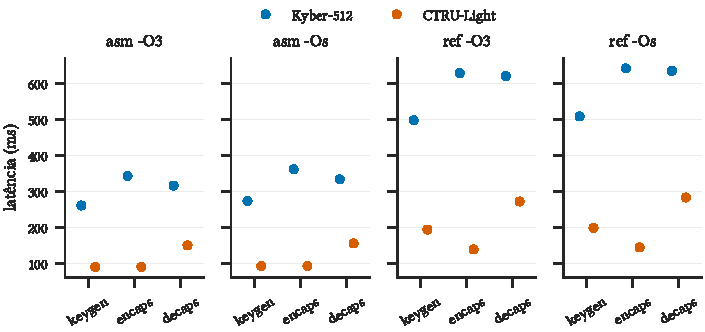
\includegraphics[width=\linewidth]{latency}
  \caption{Latência média por operação e configuração; as barras de erro
  (IC 95\%) são menores que os marcadores.}
  \Description{Quatro painéis lado a lado (asm -O3, asm -Os, ref -O3, ref
  -Os) com a latência média de KeyGen, Encaps e Decaps para Kyber-512 e
  CTRU-Light. O CTRU-Light fica abaixo do Kyber-512 em todos os painéis, e os
  painéis ref ficam cerca de duas vezes acima dos asm.}
  \label{fig:lat}
\end{figure}

Para separar a contribuição de cada fator, ajustamos o modelo linear
\begin{equation}
  \log T = \mu + \alpha_a + \beta_v + \gamma_o + \delta_p
           + (\text{interações}) + \varepsilon ,
  \label{eq:model}
\end{equation}
em que $a$, $v$, $o$ e $p$ indexam algoritmo, implementação, otimização e
operação. O logaritmo transforma efeitos multiplicativos (\emph{speedups}) em
aditivos e estabiliza a variância entre células com latências muito
diferentes. A ANOVA do modelo (Tabela~\ref{tab:anova}) mostra que o algoritmo
explica 57,8\% da soma de quadrados e a implementação, 34,0\%. A otimização do
compilador explica menos de 0,1\%. O modelo completo tem $R^2 > 0{,}99$.

\begin{table}[t]
  \caption{ANOVA (tipo II) sobre $\log T$: os seis termos de maior $\eta^2$.}
  \label{tab:anova}
  \small
  \begin{tabular}{@{}lrrr@{}}
\toprule
Termo & GL & $F$ & $\eta^2$ (\%) \\
\midrule
Algoritmo & 1 & 691.405 & 57,75 \\
Implementação & 1 & 407.358 & 34,03 \\
Operação & 2 & 26.970 & 4,51 \\
Algoritmo $\times$ Operação & 2 & 19.328 & 3,23 \\
Algoritmo $\times$ Implementação $\times$ Operação & 2 & 829 & 0,14 \\
Implementação $\times$ Operação & 2 & 746 & 0,12 \\
\midrule
Resíduo & 1476 & -- & 0,12 \\
\bottomrule
\end{tabular}

\end{table}

Comparando as alternativas par a par (razão das médias geométricas, teste de
Welch sobre $\log T$), a implementação em assembly é de 1,5 a 2,1 vezes mais
rápida que a de referência em todas as células. Já $-$Os é de 2\% a 5\% mais
lenta que $-$O3. O CTRU-Light é de 2,1 a 4,5 vezes mais rápido que o
Kyber-512, com o maior ganho no \textsf{Encaps}. Todas as diferenças têm
$p < 0{,}05$.

\subsection{Memória}
A Figura~\ref{fig:trade} cruza pico de pilha e latência. O Kyber-512 usa cerca
de 1~KB de pilha (84\% da SRAM livre, pela Eq.~\ref{eq:stack}), enquanto o
CTRU-Light usa de 2,3 a 3,2~KB (48\% a 62\% livre). A Figura~\ref{fig:flash}
mostra a Flash: as variantes de referência em $-$O3 ocupam cerca de 46~KB dos
48~KB disponíveis, e a combinação assembly com $-$Os reduz isso para 15~KB
(Kyber-512) e 23~KB (CTRU-Light).

\begin{figure}[t]
  \centering
  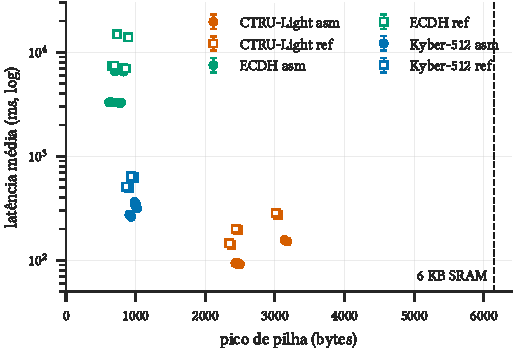
\includegraphics[width=0.62\linewidth]{tradeoff}
    \caption{Pico de pilha $\times$ latência média por operação (IC 95\%).}
    \Description{Dispersão do pico de pilha (eixo x, até o limite de 6 KB de
    SRAM, marcado por uma linha tracejada) contra a latência média. Os pontos
    do Kyber-512 ficam perto de 1 KB de pilha, com latência de 260 a 640 ms;
    os do CTRU-Light ficam entre 2,3 e 3,2 KB, com latência de 90 a 280 ms.}
    \label{fig:trade}
\end{figure}

\begin{figure}[t]
  \centering
  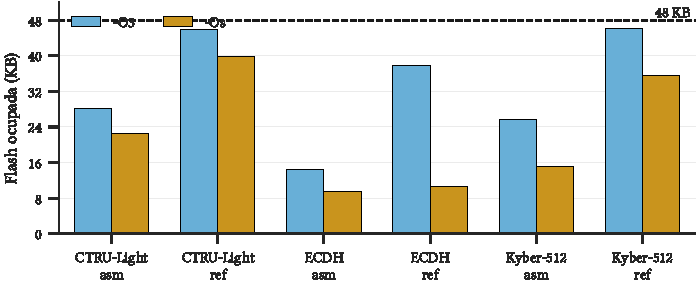
\includegraphics[width=\linewidth]{flash}
  \caption{Flash ocupada por configuração; a linha tracejada é o limite de
  48~KB do ATmega4809.}
  \Description{Barras de Flash ocupada para cada algoritmo e implementação,
  em -O3 e -Os, com uma linha tracejada no limite de 48 KB. As variantes ref
  em -O3 de Kyber-512 e CTRU-Light chegam perto do limite; as asm em -Os ocupam
  menos da metade.}
  \label{fig:flash}
\end{figure}

% ------------------------------------------------------------
\section{Discussão}
\label{sec:disc}
O fator de maior ganho sob controle do desenvolvedor é a implementação em
assembly AVR. Ela reduz a latência pela metade e, no Kyber-512 $-$O3, libera
cerca de 20~KB de Flash; sem ela, a variante de referência deixa só 4\% da
Flash para a aplicação. A otimização $-$Os é a escolha dominante no
ATmega4809: custa de 2\% a 5\% de latência, mas economiza de 6 a 11~KB num
dispositivo em que a Flash é o recurso escasso.

Entre os algoritmos há um \emph{trade-off} real. O CTRU-Light é mais rápido,
mas usa cerca de três vezes mais pilha que o Kyber-512, deixando metade da
SRAM livre em vez de 84\%. Para um nó sensor que precisa de memória para a
pilha de rede ou para um RTOS, essa diferença pode pesar mais que os
milissegundos ganhos.

O \textsf{KeyGen} e o \textsf{Encaps} do CTRU-Light têm coeficiente de
variação de 3\% a 6\% e mediana acima da média, o que sugere uma distribuição
bimodal, possivelmente por amostragem com rejeição; a causa ainda não foi
verificada no código. A cifragem da mensagem que complementa o protocolo
(um XOR simples com o segredo, idêntico em todos os firmwares e fora do KEM)
fica entre 38,4 e 39,2~ms em todas as configurações $-$O3. Como ela é quase
toda \emph{overhead} de comunicação, serve de controle de estabilidade entre
campanhas e dá uma ordem de grandeza desse \emph{overhead}.

\subsection{Limitações}
\begin{enumerate}
  \item A latência inclui o \emph{overhead} serial do host; as razões entre
        configurações são mais confiáveis que os valores absolutos. A medição
        pelo pulso GPIO no analisador lógico removerá esse viés.
  \item A ordem de execução não foi aleatorizada na bancada (cada
        configuração rodou em bloco, com ciclo fixo de operações). Efeitos
        temporais dentro de uma campanha podem, em princípio, confundir-se
        com a configuração.
  \item Só 20~MHz foi coletado, então o fator clock ainda não entra no modelo.
  \item A energia não foi medida (shunt e bateria pendentes).
  \item Não há dados de bancada do ECDH.
  \item As células são desbalanceadas ($N$ de 10 a 165).
  \item Os resíduos do modelo não são normais nas células bimodais; com $N$
        grande e efeitos dessa magnitude, as conclusões não dependem disso.
\end{enumerate}

% ------------------------------------------------------------
\section{Conclusão}
\label{sec:concl}
% TODO(autor): revisar as recomendações depois das medições de energia e clock.
Num MCU de 8~bits com 6~KB de SRAM e 48~KB de Flash, o Kyber-512 e o
CTRU-Light são viáveis em latência, com centenas de milissegundos por
operação, e deixam margem de memória para a aplicação, desde que se use a
implementação em assembly com $-$Os. A escolha entre eles é um \emph{trade-off}
entre tempo (CTRU-Light) e SRAM (Kyber-512). Os próximos passos são medir a
energia por operação, coletar os níveis de 10 e 5~MHz e incluir o ECDH como
linha de base.

% ------------------------------------------------------------
\section{Uso de ferramentas de IA}
\label{sec:ia}
Esta seção atende ao item 5.3 dos requisitos da disciplina.

\paragraph{Agente e condições de uso} Kiro (IDE com agente), modelo Claude
Opus, em modo autônomo no repositório, com tarefas pedidas uma a uma pelo
autor.
% TODO(autor): incluir outras ferramentas de IA usadas, se houver.

\paragraph{Dados fornecidos} O repositório inteiro (firmware, scripts e dados
brutos de \texttt{data/experiments/}) e o documento de requisitos.

\paragraph{Metodologia} Pedido do autor $\rightarrow$ proposta e implementação
pelo agente $\rightarrow$ revisão humana das alterações e reexecução
$\rightarrow$ integração ao repositório.

\paragraph{Verificação humana}
% TODO(autor): descrever o que foi conferido à mão (ex.: recálculo de uma
% média/IC, inspeção das figuras, revisão do texto).
\emph{A preencher pelo autor.}

\paragraph{Partes produzidas com auxílio de IA} Revisão do projeto; separação
entre dados simulados e de bancada em \texttt{run\_experiment.py};
\texttt{catalog.py}; o caderno \texttt{analise.ipynb} (código e rascunho da
interpretação); a formatação deste artigo no template ACM e o rascunho das
Seções~\ref{sec:intro} a~\ref{sec:concl}; os slides da etapa parcial.
% TODO(autor): listar demais trechos (firmware, trigger.py, etc.).

%% Agradecimentos: ambiente acks, conforme o sample (não usar \section).
\begin{acks}
% TODO(autor): agradecimentos (orientação, laboratório, etc.), se houver.
Ao Prof. Lucas Mello Schnorr, pela disciplina CMP223.
\end{acks}

\bibliographystyle{ACM-Reference-Format}
\bibliography{referencias}

%% Apêndices depois da bibliografia, conforme o sample.
\appendix
\section{Reprodutibilidade}
\label{app:repro}
Todo o material está no repositório do trabalho. Para regenerar as tabelas e
figuras deste artigo a partir dos dados brutos:
\begin{verbatim}
py -3.13 -m venv .venv
.venv\Scripts\python -m pip install -r src/analysis/requirements-notebook.txt
python src/analysis/catalog.py
.venv\Scripts\python -m jupyter nbconvert --to notebook --execute \
    --inplace src/analysis/analise.ipynb
\end{verbatim}

\end{document}
